\begin{enumerate}

\item A solid metallic sphere of radius $6$$\mathrm{cm}$ is melted and made into a solid cylinder of height $32$$\mathrm{cm}$.Find the:
	\begin{enumerate}
		\item radius of the cylinder
		\item curved surface area of the cylinder
	\end{enumerate}

\item A hemispherical and a conical hole is scooped out of a solid wooden cylinder.
Find the volume of the remaining solid where the measurements are as follows:
The height of the solid cylinder is $7\mathrm{cm}$, radius of each of hemisphere, cone and cylinder is $3\mathrm{cm}$.Height of cone is $3\mathrm{cm}$.\\
Give your answer correct to the nearest whole number. Take $\pi$ = $\frac{22}{7}$.

\begin{figure}[!ht]
		\centering
		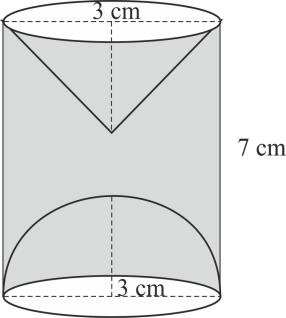
\includegraphics[width=\columnwidth]{figs/icse2.jpg}
		\caption{}
		\label{fig:enter-label}
	\end{figure}


\end{enumerate}

